\newpage

% template tabella!! Da cancellare solo quando finito
%\begin{table}[H]
%	\begin{center}
%		\begin{tabular}{|c|c|c|c|c|c|c|c|}
%			\hline
%			\textbf{nome} & \multicolumn{6}{c|}{\textbf{Ore per ruolo}} & \textbf{Ore totali} \\\cline{2-7}
%			& \textbf{Resp} & \textbf{Amm} & \textbf{An} & \textbf{Proj} & \textbf{Prog} & \textbf{Ver} & \\
%			\hline
%			\MC			&		&		&		&		&		&		&		\\
%			\hline
%			\AN			&		&		&		&	 	&		&		& 		\\
%			\hline
%			\DAN		&		&		&		&		&		&		&		\\
%			\hline
%			\AS			&		&	 	&	 	&		&	 	& 		&		\\
%			\hline
%			\NS 		&		&		&		&		&		& 		&		\\
%			\hline
%			\DS			& 		&		&		&		&		&		&		\\
%			\hline
%		\end{tabular}
%	\end{center}
%	\caption{Ore per componente, \AdR}
%\end{table}


\section{Registro suddivisione lavoro}
Nei seguenti paragrafi verrà spiegato come il gruppo intende dividere soddisfare alcune regole del progetto:
\begin{itemize}
	\item Tutti i componenti devono ricoprire almeno una volta tutti i ruoli; 
	\item Un componente del gruppo può ricoprire più ruoli contemporaneamente, a patto che non entri in conflitto d'interesse (ad esempio, non può verificare il lavoro da lui svolto).
\end{itemize}

\subsection{Periodo di Analisi dei Requisiti}
Durante il periodo di \AdR, il lavoro dei membri sarà suddiviso come segue:

\begin{table}[H]
	\begin{center}
		\begin{tabular}{|c|c|c|c|c|c|c|c|}
			\hline
			\textbf{Nome} & \multicolumn{6}{c|}{\textbf{Ore per ruolo}} & \textbf{Ore totali} \\\cline{2-7}
			& \textbf{Resp} & \textbf{Amm} & \textbf{An} & \textbf{Proj} & \textbf{Prog} & \textbf{Ver} & \\
			\hline
			\MC			&		&		&	16	&		&		&	15	&	31	\\
			\hline
			\AN			&		&	3	&	6	&	 	&		&	22	& 	31	\\
			\hline
			\DAN		&		&	3	&	29	&		&		&		&	32	\\
			\hline
			\AS			&	20	&	 	&	12 	&		&	 	& 		&	32	\\
			\hline
			\NS 		&	18	&	3	&	11	&		&		& 		&	32	\\
			\hline
			\DS			& 		&	2	&	5	&		&		&	24	&	31	\\
			\hline
		\end{tabular}
	\end{center}
	\caption{Ore per componente, \AdR}
\end{table}

\begin{figure}[H]
	\centering
	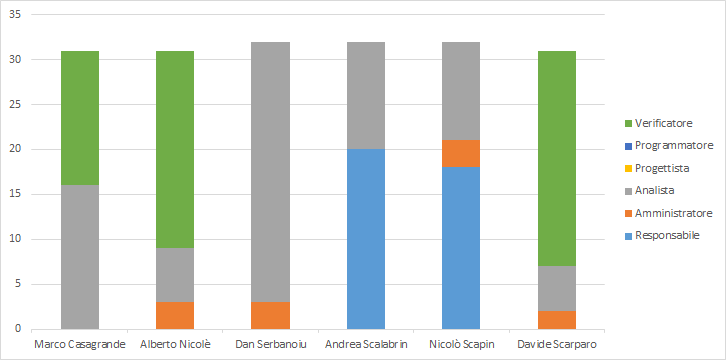
\includegraphics[scale=0.6]{img/6-1.png}
	\caption{Suddivisione ruoli per componente, Analisi dei Requisiti}
\end{figure}

\subsection{Periodo di Analisi dei Requisiti Dettagliata}
Durante il periodo di \ARD, il lavoro dei membri sarà suddiviso come segue:

\begin{table}[H]
	\begin{center}
		\begin{tabular}{|c|c|c|c|c|c|c|c|}
			\hline
			\textbf{Nome} & \multicolumn{6}{c|}{\textbf{Ore per ruolo}} & \textbf{Ore totali} \\\cline{2-7}
			& \textbf{Resp} & \textbf{Amm} & \textbf{An} & \textbf{Proj} & \textbf{Prog} & \textbf{Ver} & \\
			\hline
			\MC			&		&	1	&	 	&		&		&	2 	&	 3	\\
			\hline
			\AN			&		&		&	3 	&	 	&		&	 	& 	 3	\\
			\hline
			\DAN		&		&	 	&	2 	&		&		&		&	 2	\\
			\hline
			\AS			&	2	&	 	&	  	&		&	 	& 		&	 2	\\
			\hline
			\NS 		&	2	&		&	 	&		&		& 		&	 2	\\
			\hline
			\DS			& 		&	 	&	 	&		&		&	3 	&	 3	\\
			\hline
		\end{tabular}
	\end{center}
	\caption{Ore per componente, \ARD}
\end{table}

\begin{figure}[H]
	\centering
	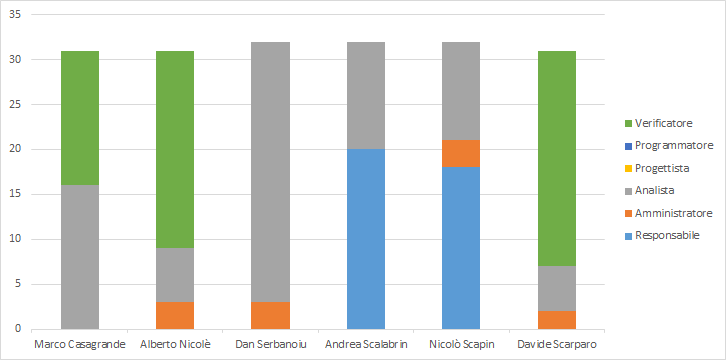
\includegraphics[scale=0.6]{img/6-1a.png}
	\caption{Suddivisione ruoli per componente, Analisi dei Requisiti Dettagliata}
\end{figure}

\subsection{Periodo di Progettazione Architetturale}
Durante il periodo di Progettazione Architetturale, il lavoro dei membri sarà suddiviso come segue:

\begin{table}[H]
	\begin{center}
		\begin{tabular}{|c|c|c|c|c|c|c|c|}
			\hline
			\textbf{Nome} & \multicolumn{6}{c|}{\textbf{Ore per ruolo}} & \textbf{Ore totali} \\\cline{2-7}
			& \textbf{Resp} & \textbf{Amm} & \textbf{An} & \textbf{Proj} & \textbf{Prog} & \textbf{Ver} & \\
			\hline
			\MC			&		&	3	&		&	31	&		&		&   34	\\
			\hline
			\AN			&	3	&		&		&	31	&		&		& 	34	\\
			\hline
			\DAN		&		&	2	&		&	17	&		&	14	&	33	\\
			\hline
			\AS			&		&	 	&	 	&	14	&	 	& 	19	&	33	\\
			\hline
			\NS 		&		&		&		&	14	&		& 	19	&	33	\\
			\hline
			\DS			& 	2	&		&		&	31	&		&		&	33	\\
			\hline
		\end{tabular}
	\end{center}
	\caption{Ore per componente, Progettazione Architetturale}
\end{table}

\begin{figure}[H]
	\centering
	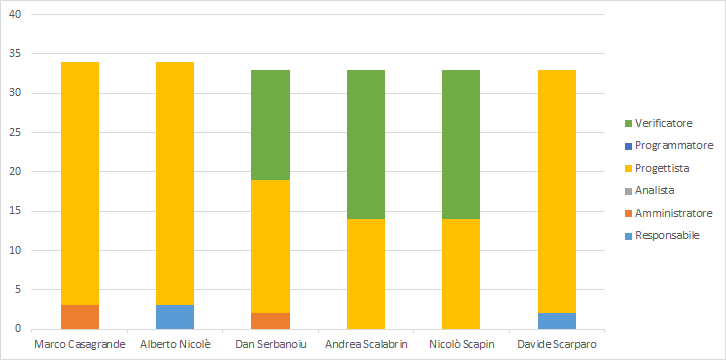
\includegraphics[scale=0.6]{img/6-2.png}
	\caption{Suddivisione ruoli per componente, Progettazione Architetturale}
\end{figure}

\subsection{Periodo di Progettazione Architetturale Dettagliata}
Durante il periodo di progettazione architetturale, il lavoro dei membri sarà suddiviso come segue:

\begin{table}[H]
	\begin{center}
		\begin{tabular}{|c|c|c|c|c|c|c|c|}
			\hline
			\textbf{Nome} & \multicolumn{6}{c|}{\textbf{Ore per ruolo}} & \textbf{Ore totali} \\\cline{2-7}
			& \textbf{Resp} & \textbf{Amm} & \textbf{An} & \textbf{Proj} & \textbf{Prog} & \textbf{Ver} & \\
			\hline
			\MC			&	2	&		&		&	6	&		&	11	&	19	\\
			\hline
			\AN			&		&		&		&	8	&   	&	11	& 	19	\\
			\hline
			\DAN		&	3	&		&		&	17	&		&		&	20	\\
			\hline
			\AS			&		&	3	&	 	&	17	&	 	& 		&	20	\\
			\hline
			\NS 		&		&	3	&		&	17	&		& 		&	20	\\
			\hline
			\DS			& 		&		&		&	7	&		&	13	&	20	\\
			\hline
		\end{tabular}
	\end{center}
	\caption{Ore per componente, Progettazione Architetturale Dettagliata}
\end{table}

\begin{figure}[H]
	\centering
	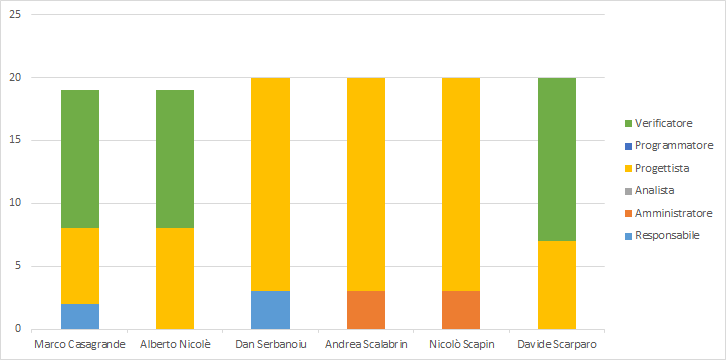
\includegraphics[scale=0.6]{img/6-3.png}
	\caption{Suddivisione ruoli per componente, Progettazione Architetturale Dettagliata}
\end{figure}

\subsection{Periodo di Codifica}
Durante il periodo di Codifica, il lavoro dei membri sarà suddiviso come segue:

\begin{table}[H]
	\begin{center}
		\begin{tabular}{|c|c|c|c|c|c|c|c|}
			\hline
			\textbf{Nome} & \multicolumn{6}{c|}{\textbf{Ore per ruolo}} & \textbf{Ore totali} \\\cline{2-7}
			& \textbf{Resp} & \textbf{Amm} & \textbf{An} & \textbf{Proj} & \textbf{Prog} & \textbf{Ver} & \\
			\hline
			\MC			&		&		&		&		&	18	&	18	&	36	\\
			\hline
			\AN			&	3	&		&		&	 	&	32	&		& 	35	\\
			\hline
			\DAN		&		&		&		&		&	14	&	21	&	35	\\
			\hline
			\AS			&		&	 	&	 	&		&	14 	& 	22	&	36	\\
			\hline
			\NS 		&		&	3	&		&		&	32	& 		&	35	\\
			\hline
			\DS			& 	3	&		&		&		&	33	&		&	36	\\
			\hline
		\end{tabular}
	\end{center}
	\caption{Ore per componente, Codifica}
\end{table}

\begin{figure}[H]
	\centering
	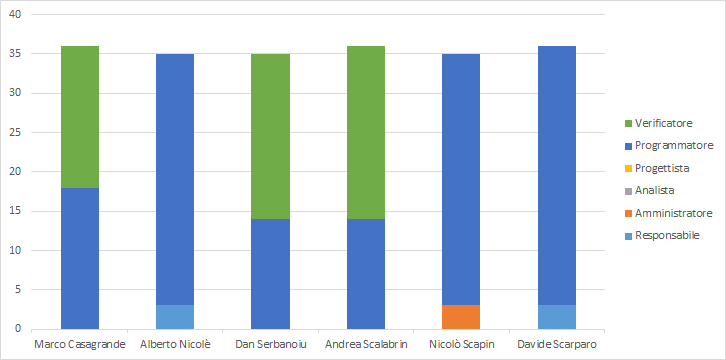
\includegraphics[scale=0.6]{img/6-4.png}
	\caption{Suddivisione ruoli per componente, Codifica}
\end{figure}

\subsection{Periodo di Verifica e Validazione}
Durante il periodo di Verifica e Validazione, il lavoro dei membri sarà suddiviso come segue:

\begin{table}[H]
	\begin{center}
		\begin{tabular}{|c|c|c|c|c|c|c|c|}
			\hline
			\textbf{Nome} & \multicolumn{6}{c|}{\textbf{Ore per ruolo}} & \textbf{Ore totali} \\\cline{2-7}
			& \textbf{Resp} & \textbf{Amm} & \textbf{An} & \textbf{Proj} & \textbf{Prog} & \textbf{Ver} & \\
			\hline
			\MC			&		&	3	&		&	7	&		&	6	&	16	\\
			\hline
			\AN			&		&		&		&	 	&		&	17	& 	17	\\
			\hline
			\DAN		&	3	&		&		&		&		&	14	&	17	\\
			\hline
			\AS			&		&	 	&	 	&	4	&	 	& 	12	&	16	\\
			\hline
			\NS 		&		&		&		&	4	&		& 	13	&	17	\\
			\hline
			\DS			& 		&		&		&		&		&	16	&	16	\\
			\hline
		\end{tabular}
	\end{center}
	\caption{Ore per componente, Verifica}
\end{table}

\begin{figure}[H]
	\centering
	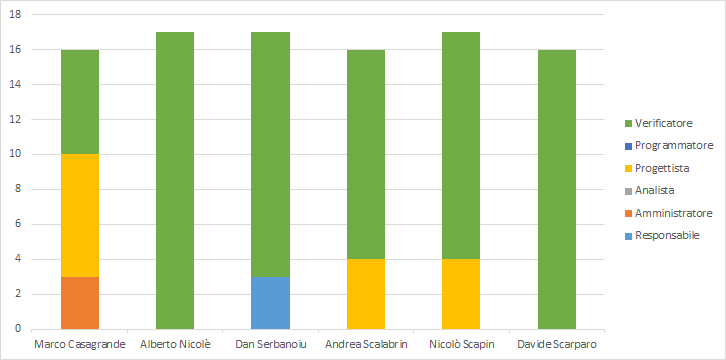
\includegraphics[scale=0.6]{img/6-5.png}
	\caption{Suddivisione ruoli per componente, Verifica}
\end{figure}

\subsection{Ore totali per componente}
Il consuntivo delle ore totali, raggruppate per ciascun membro del gruppo, e suddiviso per il ruolo assunto durante tutte le fasi del progetto, risulta essere così suddiviso:

\begin{table}[H]
	\begin{center}
		\begin{tabular}{|c|c|c|c|c|c|c|c|}
			\hline
			\textbf{Nome} & \multicolumn{6}{c|}{\textbf{Ore per ruolo}} & \textbf{Ore totali} \\\cline{2-7}
			& \textbf{Resp} & \textbf{Amm} & \textbf{An} & \textbf{Proj} & \textbf{Prog} & \textbf{Ver} & \\
			\hline
			\MC			&	2	&	7	&	16	&	44	&	18	&	52	&	139	\\
			\hline
			\AN			&	6	&	4	&	9	&	39	&	32	&	50	& 	139	\\
			\hline
			\DAN		&	6	&	4	&	32	&	34	&	14	&	49	&	139	\\
			\hline
			\AS			&	22	&	3 	&	12 	&	35	&	14 	& 	53	&	139	\\
			\hline
			\NS 		&	20	&	9	&	11	&	35	&	32	& 	32	&	139	\\
			\hline
			\DS			& 	5	&	2	&	5	&	38	&	33	&	57	&	139	\\
			\hline
		\end{tabular}
	\end{center}
	\caption{Ore totali, per componente}
\end{table}

\subsection{Ore totali remunerabili}
La tabella sottostante, infine, raccoglie il conteggio complessivo delle ore remunerabili, suddivise per ruolo e componente.

\begin{table}[H]
	\begin{center}
		\begin{tabular}{|c|c|c|c|c|c|c|c|}
			\hline
			\textbf{Nome} & \multicolumn{6}{c|}{\textbf{Ore per ruolo}} & \textbf{Ore totali} \\\cline{2-7}
			& \textbf{Resp} & \textbf{Amm} & \textbf{An} & \textbf{Proj} & \textbf{Prog} & \textbf{Ver} & \\
			\hline
			\MC			&	2	&	6	&	0	&	44	&	18	&	35	&	105	\\
			\hline
			\AN			&	6	&	0	&	0	&	39	&	32	&	28	& 	105	\\
			\hline
			\DAN		&	6	&	2	&	0	&	34	&	14	&	49	&	105	\\
			\hline
			\AS			&	0	&	3 	&	0 	&	35	&	14 	& 	53	&	105	\\
			\hline
			\NS 		&	0	&	6	&	0	&	35	&	32	& 	32	&	105	\\
			\hline
			\DS			& 	5	&	0	&	0	&	38	&	33	&	29	&	105	\\
			\hline
		\end{tabular}
	\end{center}
	\caption{Ore totali remunerabili, per ruolo e componente}
\end{table}
